\documentclass[twoside]{article}
\setlength{\oddsidemargin}{0.25 in}
\setlength{\evensidemargin}{-0.25 in}
\setlength{\topmargin}{-0.6 in}
\setlength{\textwidth}{6.5 in}
\setlength{\textheight}{8.5 in}
\setlength{\headsep}{0.75 in}
\setlength{\parindent}{0 in}
\setlength{\parskip}{0.1 in}
\usepackage{subcaption}

\usepackage{graphicx}
\usepackage{url}

%
% The following commands sets up the lecnum (lecture number)
% counter and make various numbering schemes work relative
% to the lecture number.
%
\newcounter{lecnum}
\renewcommand{\thepage}{\thelecnum-\arabic{page}}
\renewcommand{\thesection}{\thelecnum.\arabic{section}}
\renewcommand{\theequation}{\thelecnum.\arabic{equation}}
\renewcommand{\thefigure}{\thelecnum.\arabic{figure}}
\renewcommand{\thetable}{\thelecnum.\arabic{table}}
\newcommand{\dnl}{\mbox{}\par}

%
% The following macro is used to generate the header.
%
\newcommand{\lecture}[4]{
  \pagestyle{myheadings}
  \thispagestyle{plain}
  \newpage
  \setcounter{lecnum}{#1}
  \setcounter{page}{1}
  \noindent
  \begin{center}
  \framebox{
     \vbox{\vspace{2mm}
   \hbox to 6.28in { {\bf CMPSCI~630~~~Systems
                       \hfill Fall 2019} }
      \vspace{4mm}
      \hbox to 6.28in { {\Large \hfill Lecture #1  \hfill} }
%       \hbox to 6.28in { {\Large \hfill Lecture #1: #2  \hfill} }
      \vspace{2mm}
      \hbox to 6.28in { {\it Lecturer: #3 \hfill Scribe: #4} }
     \vspace{2mm}}
  }
  \end{center}
  \markboth{Lecture #1: #2}{Lecture #1: #2}
  \vspace*{4mm}
}

%
% Convention for citations is authors' initials followed by the year.
% For example, to cite a paper by Leighton and Maggs you would type
% \cite{LM89}, and to cite a paper by Strassen you would type \cite{S69}.
% (To avoid bibliography problems, for now we redefine the \cite command.)
%
\renewcommand{\cite}[1]{[#1]}

% \input{epsf}

%Use this command for a figure; it puts a figure in wherever you want it.
%usage: \fig{NUMBER}{FIGURE-SIZE}{CAPTION}{FILENAME}
\newcommand{\fig}[4]{
           \vspace{0.2 in}
           \setlength{\epsfxsize}{#2}
           \centerline{\epsfbox{#4}}
           \begin{center}
           Figure \thelecnum.#1:~#3
           \end{center}
   }

% Use these for theorems, lemmas, proofs, etc.
\newtheorem{theorem}{Theorem}[lecnum]
\newtheorem{lemma}[theorem]{Lemma}
\newtheorem{proposition}[theorem]{Proposition}
\newtheorem{claim}[theorem]{Claim}
\newtheorem{corollary}[theorem]{Corollary}
\newtheorem{definition}[theorem]{Definition}
\newenvironment{proof}{{\bf Proof:}}{\hfill\rule{2mm}{2mm}}

% Some useful equation alignment commands, borrowed from TeX
\makeatletter
\def\eqalign#1{\,\vcenter{\openup\jot\m@th
 \ialign{\strut\hfil$\displaystyle{##}$&$\displaystyle{{}##}$\hfil
     \crcr#1\crcr}}\,}
\def\eqalignno#1{\displ@y \tabskip\@centering
 \halign to\displaywidth{\hfil$\displaystyle{##}$\tabskip\z@skip
   &$\displaystyle{{}##}$\hfil\tabskip\@centering
   &\llap{$##$}\tabskip\z@skip\crcr
   #1\crcr}}
\def\leqalignno#1{\displ@y \tabskip\@centering
 \halign to\displaywidth{\hfil$\displaystyle{##}$\tabskip\z@skip
   &$\displaystyle{{}##}$\hfil\tabskip\@centering
   &\kern-\displaywidth\rlap{$##$}\tabskip\displaywidth\crcr
   #1\crcr}}
\makeatother

% **** IF YOU WANT TO DEFINE ADDITIONAL MACROS FOR YOURSELF, PUT THEM HERE:



% Some general latex examples and examples making use of the
% macros follow.

\begin{document}

%FILL IN THE RIGHT INFO.
%\lecture{**LECTURE-NUMBER**}{**DATE**}{**LECTURER**}{**SCRIBE**}
\lecture{12}{October 29}{Emery Berger}{Mehmet Savasci, Vincent Pun}

We continued discussions on microkernels and monolithic kernels.

\section{Microkernels vs Monolithic Kernels}

\subsection{Exokernels}

Exokernels are a follow-on to microkernels. They move as much functionality out of a normal operating system as possible, since the OS has direct access to hardware and is hence potentially dangerous. If anything goes wrong in a process, it is terminated without affecting the entire kernel.

Exokernels have the benefits of a microkernel inside a monolithic kernel. They are made possible using virtual memory protection. Each process has an isolated memory area, in the same vein as microkernels.

\subsection{Performance}

Microkernels have processes communicating with the kernel. However, these communications are expensive as they involve copying and context switches.

For example, suppose a process needs to write data into a file. In a microkernel, the data is copied to the process that handles file I/O, and another copy is then made into the kernel, resulting in a 2x memory overhead. In a monolithic kernel, the data gets copied into the kernel and writes it to the file.

There is also a context switch every time a microkernel process communicates with the kernel. For example, the file I/O process may have to communicate with the virtual memory management process. This comes with the costs of context switches: clearing registers, flushing the TLB, warming the cache, and so on. In contrast, the monolithic kernel can achieve this by simply invoking functions because these units share the same space, which is practically free.

\subsection{Microkernels and Monolithic Kernels Today}

CMU developed the Mach microkernel. The Mach microkernel led to OS X and iOS. However, in OS X and iOS, all of the microkernel components are compiled into a monolithic kernel. In essence, the OS X and iOS kernels are micro from a software engineering standpoint.

People from the Netherlands developed the MINIX microkernel, which continues to exist today.

Microkernels are regarded as safe, whereas monolithic kernels are fast. The monotholic kernel approach clearly won thanks to its performance, as most operating systems widely in use such as Windows, Linux, and OS X are all monolithic kernels.

\section{Containers and Virtual Machines}

Today, discussions around boxing these units have moved up a level to containers and virtual machines, which create one unit of indirection. Virtual machines are operating systems on a layer which pretends to be a computer. VMs were invented by IBM because of a demand to run old software on new hardware. Figures \ref{fig:architecture-prev} and \ref{fig:architecture-now} show the differences.

While the virtual machines structure may appear slow, the VMs are in actuality dynamically JIT-ing the code.

\begin{figure}
\centering
\begin{minipage}{.6\textwidth}
  \centering
  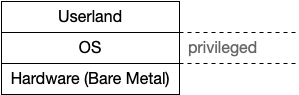
\includegraphics[width=.7\linewidth]{architecture-prev}
  \captionof{figure}{Previous structure. Note that the OS can be a microkernel or a monolithic kernel.}
  \label{fig:architecture-prev}
\end{minipage}%
\begin{minipage}{.4\textwidth}
  \centering
  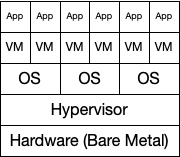
\includegraphics[width=.6\linewidth]{architecture-now}
  \captionof{figure}{Today's structure.}
  \label{fig:architecture-now}
\end{minipage}
\end{figure}

\subsection{Support in Software and Hardware}

It is necessary to map the virtual \textit{physical} memory inside the VM to the actual physical memory. Originally, this is performed in software: the software stops at each virtual physical memory address access, finds the actual memory address and returns it to the program. This is slow.

IBM hardware provides hardware support, by allowing separate physical memory mappings, which is fast.

The Intel architecture was thought to be practically unvirtualizable. Mendel Rosenblum invented practical virtualization for Intel. The VMs dynamically JIT-compile code by replacing reads and writes to actual memory addresses and turning privileged instructions to system calls. Commonly executed chunks of code are compiled one-time, future runs are at full-speed. Mendel and his wife went on to start VMware.

Intel and AMD now have hardware extensions for virtualization years later. Fast switching TLB is now supported in hardware. However, VMware claims their approach is faster.

\subsection{Paravirtualization}

Paravirtualization is VMs crossing the boundary straight to the host OS without having to wrap calls through the VM.

VMware is fast because of paravirtualization. It has custom drivers for that directly communicate with hardware. For example, the graphics card driver allows GPU writes to directly jump down to the hardware. Browsers also contain paravirtualization. Writing things into canvases in JavaScript turns into calls that directly go to the GPU, because canvases are a shortcut to the GPU.

\section{Security}

\subsection{Attacks}

\textit{Asymmetric attack} is a kind of attacks that gives one side more power than the other. \textit{Symmetric attack} is a kind of attacks where there is an equivalent amount of opposing force. Security exploits typically lead to asymmetric attacks.

\subsection{Confinement}

Confinement enforcement can be done on different levels: hardware, OS, and software.

\subsubsection{Software-level Enforcement}

\paragraph{Device Drivers}

Device drivers in operating systems are potentially dangerous because they directly communicate with devices. They can write arbitrary data to devices, and can read arbitrary data from devices. Therefore device driver code must be carefully written.

Direct memory access (DMA) is fast as it allows data to be directly written to the memory from the device. For example, a network card (NIC) can write packet from the Internet directly to the RAM without having to involve buffer copying through software. This is risky because the device has access to the entire memory, an error could write into the kernel code. There is also remote DMA (RDMA), which allows direct access to other computers in a network, typically used in a rack setting.

OS kernels kill themselves when an internal integrity check fails or a hardware error is discovered. In Windows, this results in blue screen of death (BSOD), and in Linux, this results in a kernel panic. Bad device drivers used to be the primary source of bugs in Windows.

Microsoft attempted to remedy this situation by requiring drivers to be signed, which required driver writers to pay for a certificate to sign the drivers. Windows would show a warning dialog when an unsigned device driver is about to be installed.

Microsoft now provides a new API for device drivers with a driver development kit (DDK) to develop device drivers. The development kit includes a static analyzer which enforces security checks.

\subsubsection{OS-level Enforcement}

\paragraph{Browsers}

Browsers like Chrome put each tab in its own process, achieving process-level isolation. For example, plugins (device driver-equivalent in the browser world) could fail. When this happens, the pages for the one tab is taken down instead of the entire operating system. It leverages the fact that memory of processes are isolated in the OS.

\paragraph{iOS}

All applications live in their own subdirectories. When an application runs, {\tt chroot} is run to switch \texttt{/} to the subdirectory to cut off the application's access to their parent directories. In addition, each application is its own user and each file is owned by that user. In other words, it takes advantage of OS-level privileges. To access something else, explicit permission by the user is required through discretionary access control. iOS has gradually opened up.

\paragraph{Android}

Android did not have separate user processes and used to allow applications to run anything. All permissions were granted at install time. It was a reputation-based approach, which is bad from a security standpoint. Now Android is gradually revising this approach.

\subsubsection{Hardware-level Enforcement}

The TLB is hardware-level enforcement. There are other mechanisms in the hardware, but they turn out to be not as robust as people once thought.

\end{document}
